\documentclass[12pt,a4paper]{article}
\usepackage{graphicx}
\usepackage{polski}
\usepackage[utf8]{inputenc}
\title{Sprawozdanie z laboratorium PAMSI}
\author{Damian Oleksak}
\date{}
\begin{document}
\maketitle

Kolejka (bufor) jest strukturą typu FIFO (ang. First In First Out), w której odczyt następuje tylko 
z pierwszej pozycji, a wstawienie nowego elementu może nastąpić tylko na koniec struktury 
(za ostatni element). Zatem dostęp (pobranie) oraz wstawienie nowego elementu zajmuje O(1)
czasu, natomiast wyszukanie i usunięcie konkretnego elementu - O(n).

Stos jest strukturą typu LIFO (ang. Last In First Out), czyli taką, w której dostęp (bezpośredni)
jest tylko do pierwszego elementu, a dodanie nowego następuje przed pierwszy (na pierwszą pozycję). Zatem - tak jak w przypadku kolejki - złożoność operacji dostępu (pobrania) oraz dodania elementu wynosi O(1), natomiast dla wyszukania i usunięcia konkretnego elementu 
to O(n).

Wyżej wymienione struktury danych można zaimplementować przy pomocy tablicy dynamicznej lub listy. Użycie tablicy wymaga ponownego alokowania pamięci przy każdej zmianie liczby jej elementów. Przepisanie danych do tablicy tymczasowej, utworzenie nowej (większej o 1 element) i umieszczenie większej liczby danych zwiększa złożoność obliczeniową. 

Powszechnie stosowanym rozwiązaniem jest podwojenie rozmiaru tablicy, gdy liczba jej elementów ma wykroczyć poza zakres. Przy zmniejszaniu tablicy stosuje się analogiczną
operację - redukowanie rozmiaru do 1/4.

\includegraphics[width = 400pt, height = 300pt]{wy1}

Wykres 1. Każdorazowa zmiana rozmiaru tablicy o 1 element \newline

\includegraphics[width = 400pt, height = 300pt]{wy2}

Wykres 2. Dwukrotne powiększanie tablicy \newline

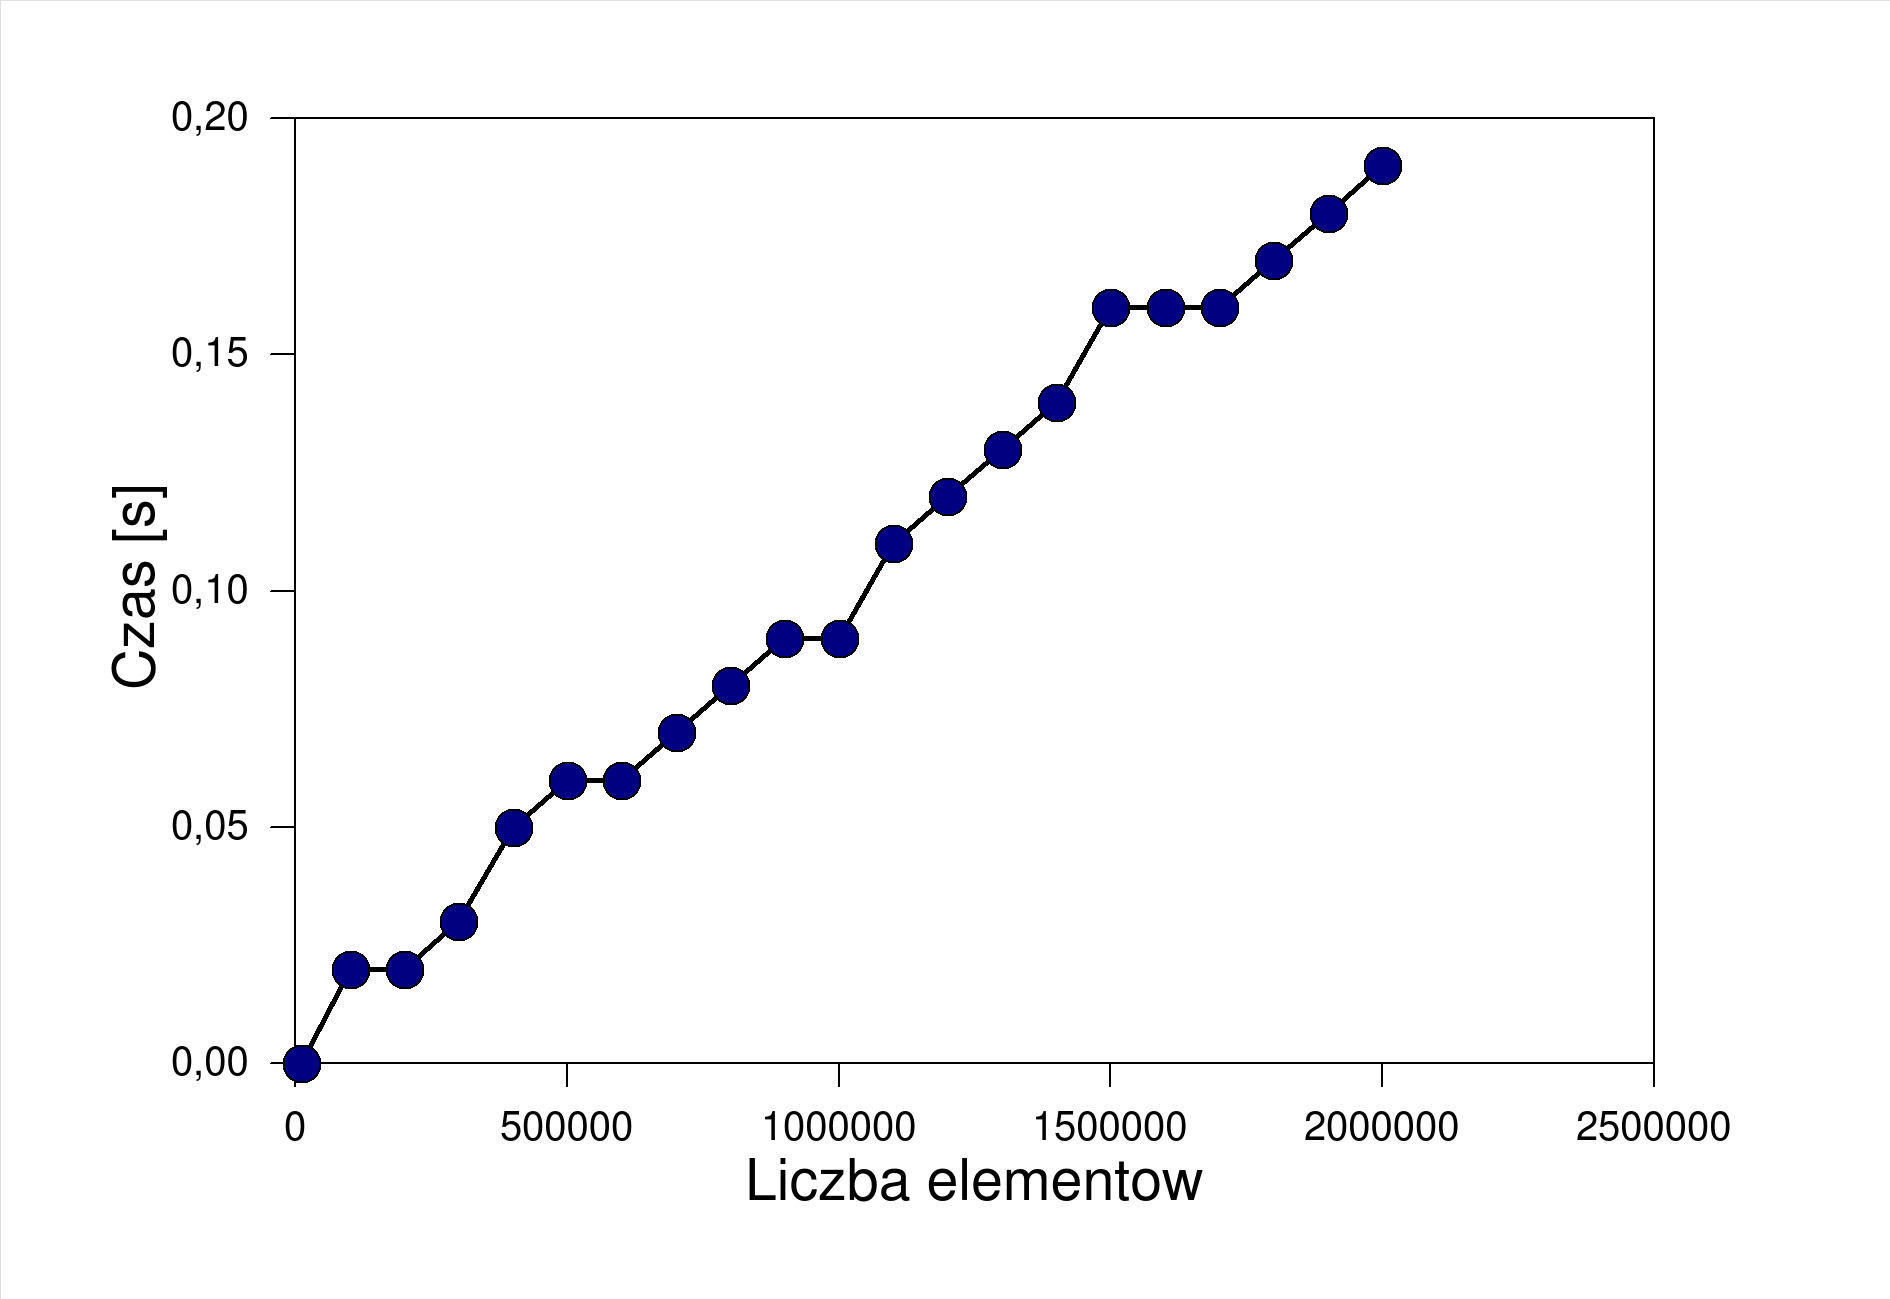
\includegraphics[width = 400pt, height = 300pt]{wy}

Wykres 3. Implementacja przy użyciu listy \newline

Wykresy zostały wygenerowane na podstawie pomiarów czasu wypełniania struktury danych od liczby jej elementów. Pierwszy wykres przedstawia złożoność kwadratową, jaką generuje pierwsze rozwiązanie. Złożoność liniowa, którą możemy zaobserwować na drugim wykresie, pozwala na operację w rozsądnym czasie na znacznie większej ilości argumentów .
Na trzecim wykresie przedstawiono wyniki osiągnięte przy rozwiązaniu problemu za pomocą listy. Złożoność obliczeniowa także jest liniowa, lecz prosta ma mniejsze nachylenie, co pozwala na szybsze dodawanie większej liczby argumentów.    \newline

\end{document} 
